Gravitons could be produced in proton-proton collisions at the \gls{lhc}. The
interaction Lagrangian is given by~\cite{ADDPhenomenology}:
\begin{equation}
  \label{eq:114}
  \mathcal{L} = - \frac{1}{\overbar{M}_P} G^{(n)}_{\mu\nu} T^{\mu\nu}
\end{equation}
where $\overbar{M}_P = M_P/\sqrt{8 \pi}$ is the reduced Planck mass,
$G^{(n)}_{\mu\nu}$ is the graviton field and $T^{\mu\nu}$ is the stress-energy
tensor, and thus the graviton production cross section is suppressed by a factor
$1/\overbar{M}^2_P$. Nevertheless the mass splitting of the Kaluza-Klein modes
is given by~\cite{ADDPhenomenology}:
\begin{equation}
  \label{eq:115}
  \Delta m \approx \frac{1}{R} = \md \left( \frac{\md}{\overbar{M}_P}
  \right)^{2/n} \approx \left( \frac{\md}{\mathrm{TeV}} \right)^{\frac{n +
  2}{2}} 10^{\frac{12 n - 31}{n}}~\mathrm{eV}
\end{equation}
where $n$ represents the extra dimensions which for $\md = 1$~TeV and $n =$ 4,
6, 8 gives $\Delta m = 20$~KeV, 7~MeV and 0.1~GeV. For $n > 6$ only few \gls{kk}
modes can be produced and the total production cross section becomes
negligible~\cite{ADDPhenomenology} while for $n \lesssim 6$ the mass splitting
energy becomes comparable with the experimental energy resolution and the number
of \gls{kk} modes produces is capable of compensating the $1/\overbar{M}^2_p$
suppression factor in the production cross section. The graviton lifetime of
$\tau_G \approx \overbar{M}^2_P/m^3 \approx (\mathrm{TeV}/m)^3 \approx
10^3$~seconds make it stable over ATLAS detection time. The $1/\overbar{M}^2_p$
suppression factor can be interpreted as the low probability that a graviton
propagating in the extra dimensions crosses the usual three spatial
dimensions. The Kaluza-Klein graviton only interacts weakly through the
gravitational interaction with the Standard Model particles and thus behaves
like a non interacting, massive and stable particle which, escaping detection,
leads to an energy imbalance in the detector which can be investigated using the
monojet signature. \cref{fig:add_feynman} shows the three main graviton
production modes at \gls{lhc}.

As mentioned earlier, \gls{add} scenarios with more than six extra dimensions do
not offer sensitivity to collider searches, for this reason in this analysis
only models with six or less extra dimensions are considered. Moreover, since
from \cref{eq:69}, using n = 1 leads to $R \approx 10^{11}$~m which is
empirically excluded models with more than two extra dimensions are
considered. Finally in the case with two and three extra dimensions, values of
$\md$ lower than 110~TeV and 5~TeV respectively are excluded by cosmological
arguments~\cite{ADDCosmology}.

In this analysis limits on $\md$ are set using its relation with the production
cross section~\cite{ADDPhenomenology}:
\begin{equation}
  \label{eq:116}
  \sigma = \frac{C_n}{\md^{n + 2}}
\end{equation}
where $C_n$ is a constant term for a given center of mass energy and number of
extra dimensions and the definition of signal strength
$\mu_\mathrm{sig} = \sigma/\sigma_\mathrm{SM}$ where $\sigma$ is the production
cross section of some \gls{bsm} model:
\begin{equation}
  \label{eq:117}
  \md^\mathrm{excl} = \frac{\md^\mathrm{nom}}{\mu^{1/(n + 2)}_\mathrm{sig}}
\end{equation}
where $\md^\mathrm{nom}$ is the fundamental Planck scale associated with the
production cross section of the \gls{mc} samples. With this prescription upper
limits on the signal strength are translated into upper limits on the
fundamental Planck scale $\md$.

\begin{figure}[!h]
  \centering
  \begin{subfigure}{.48\linewidth}
    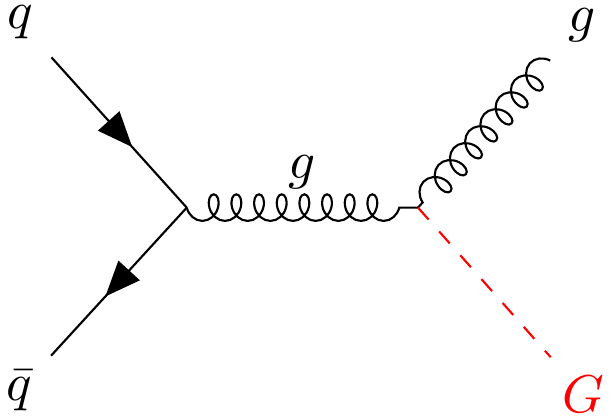
\includegraphics[width=\linewidth]{qq_to_gG}
    \caption{$q \bar{q} \rightarrow g G$.}
  \end{subfigure}
  \begin{subfigure}{.48\linewidth}
    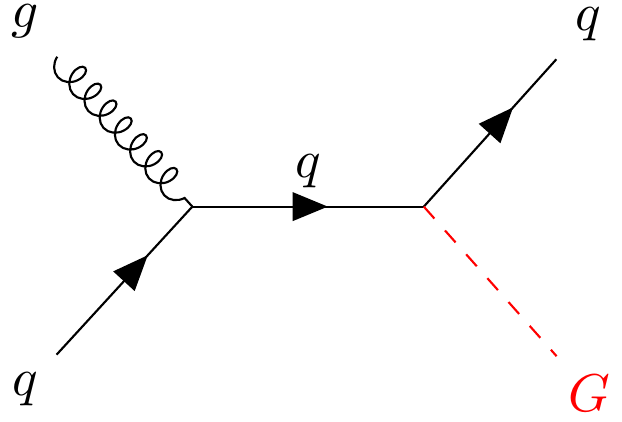
\includegraphics[width=\linewidth]{qg_to_qG}
    \caption{$q g \rightarrow q G$.}
  \end{subfigure}
  \begin{subfigure}{.48\linewidth}
    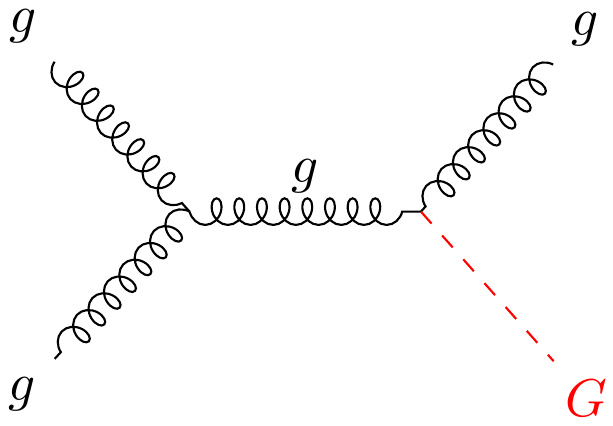
\includegraphics[width=\linewidth]{gg_to_gG}
    \caption{$g g \rightarrow g G$.}
  \end{subfigure}
  \caption{The main s-channel graviton production mechanisms for the \gls{add}
    model at \gls{lhc}.}
  \label{fig:add_feynman}
\end{figure}
%%% Local Variables:
%%% mode: latex
%%% TeX-master: "../search_for_DM_LED_with_ATLAS"
%%% End:
